\section{Связь проверки гипотез с доверительными интервалами и бутстрепом}

Существует тесная связь между проверкой гипотез и доверительными интервалами. Предположим, что наблюдаемое значение интересующей статистики $\hat{\theta}$ больше нуля. Выберем $\alpha$ так, чтобы $\hat{\theta}_{lo}$, нижний предел доверительного интервала $1-2\alpha$ для $\theta$, в точности равнялся 0.\\
\noindent
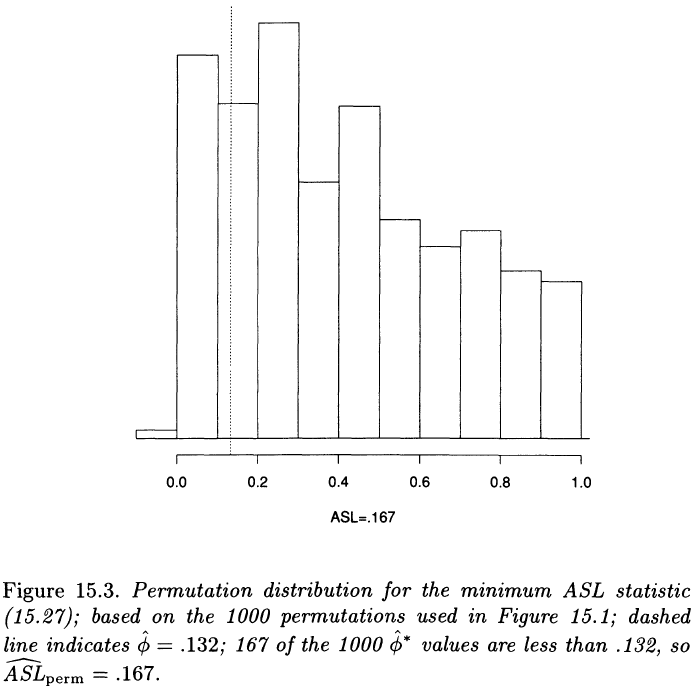
\includegraphics[width=\linewidth]{15/f15.3.png}
\newline\\
\noindent Тогда $\text{Prob}_{\theta=0}\{ \hat{\theta}^* \geq \hat{\theta} \} = \alpha$ согласно (12.13). Однако если $\theta = 0$ --- нулевая гипотеза, как в примере с данными о мышах, то определение (15.4) дает ASL = $\alpha$. Например, если 0.94 доверительный интервал $[\hat{\theta}_{lo}, \hat{\theta}_{up}]$ имеет $\hat{\theta}_{lo} = 0$, тогда ASL наблюдаемого значения $\hat{\theta}$ должен быть равен 0.03 (поскольку $0.94 = 1 - 2 \cdot 0.03$).

Другими словами, мы можем использовать доверительные интервалы для вычисления ASL. Имея это в виду, на рисунке 15.4 показано бутстреп распределение двух статистик, которые мы можем использовать для формирования доверительных интервалов для разницы между экспериментальной и контрольной группами, разности средних $\hat{\theta}_0 = \bar{z} - \bar{y}$ (левая часть рисунка), и 0.25 отсеченных разностей средних $\hat{\theta}_{0.25} = \bar{z}_{0.25} - \bar{y}_{0.25}$ (правая часть рисунка). Какое значение $\alpha$ сделает нижний предел бутстреп доверительного интервала равным нулю? Для бутстреп метода процентилей, примененного к статистике $\hat{\theta}^*$, ответ составляет
\begin{equation}
	\alpha_0 = \# \{ \hat{\theta}^*(b) < 0 \}/B,
\end{equation}
доля бутстреп репликаций меньше нуля. (Тогда $\hat{\theta}_{lo} = \hat{\theta}^*_{\alpha 0} = 0$ согласно (13.5).) Согласно предыдущему абзацу ASL $\hat{\theta}$ равно $\alpha_0$, скажем
\begin{equation}
	\widehat{\text{ASL}}_{\%} = \#\{\hat{\theta}^*(b)<0\}/B.
\end{equation}
$B = 1000$ бутстреп репликации, показанные на рис. 15.4, дали
\begin{equation}
	\widehat{\text{ASL}}_{\%}(\hat{\theta}_0) = 0.132 \quad \text{и} \quad \widehat{\text{ASL}}_{\%}(\hat{\theta}_{0.25}) = 0.180.
\end{equation}
Обратите внимание, насколько эти результаты похожи на $\widehat{\text{ASL}}_{\text{perm}} (\hat{\theta}_{0}) = 0.132$, $\widehat{\text{ASL}}_{\text{perm}} (\hat{\theta}_{0.25}) = 0.152$, рисунок 15.1.

Для доверительных интервалов $\text{BC}_{\alpha}$ для главы 14 расчет ASL дает
\begin{equation}
	\widehat{\text{ASL}}_{\text{BC}_{\alpha}} = \Phi^{-1} \left( \dfrac{\omega_0 - \hat{z}_0}{1 + \hat{\alpha}(\omega_0 - \hat{z}_0)} \right),
\end{equation}
где
\begin{equation}
	\omega_0 = \Phi^{-1}(\alpha_0)
\end{equation}
и константа коррекции смещения $\hat{z}_0$ аппроксимируется согласно формуле (14.14). Эта формула дала $\hat{z}_0 = -0.040$ для $\hat{\theta}_0$ и $\hat{z}_0 = 0.035$ для $\hat{\theta}_{0.25}$.

Константа ускорения $\hat{\alpha}$ определяется двухвыборочной версией формулы (14.15). Пусть $\hat{\theta}_{z,(i)}$ будет значением $\hat{\theta}$, когда мы исключаем $z_i$, и $\hat{\theta}_{y,(i)}$ будет значением $\hat{\theta}$, когда мы исключаем $y_i$. Пусть 
$$\hat{\theta}_{z,(\cdot)} = \sum\limits_{1}^{n} \hat{\theta}_{z,(i)}/n,$$
$$\hat{\theta}_{y,(\cdot)} = \sum\limits_{1}^{m} \hat{\theta}_{y,(i)}/m,$$
$$U_{z,i} = (n-1)(\hat{\theta}_{z,(\cdot)} - \hat{\theta}_{z,(i)}),$$
$$U_{y,i} = (m-1)(\hat{\theta}_{y,(\cdot)} - \hat{\theta}_{y,(i)}).$$
Тогда
\begin{equation}
	\hat{\alpha} = \dfrac{1}{6} \dfrac{[\sum_{i=1}^n U_{z,i}^{3} / n^3 + \sum_{i=1}^m U_{y,i}^3 / m^3]}{[\sum_{i=1}^n U_{z,i}^2 /n^2 + \sum_{i=1}^m U_{y,i}^2 / m^2]^{3/2}},
\end{equation}
$n$ и $m$ --- длины $\bf{z}$ и $\bf{y}$. Формула (15.36) дает $\hat{\alpha} = 0.06$ и $\hat{\alpha} = -0.01$ для $\hat{\theta}_0$ и $\hat{\theta}_{0.25}$ соответственно. Тогда
\begin{equation}
	\widehat{\text{ASL}}_{\text{BC}_{\text{a}}}(\hat{\theta}_0) = 0.147 \quad \text{и} \quad \widehat{\text{ASL}}_{\text{BC}_{\text{a}}}(\hat{\theta}_{0.25}) = 0.167
\end{equation}
согласно (15.34).

Вот некоторые моменты, о которых следует помнить при сравнении рисунков 15.1 и 15.4:

\noindent
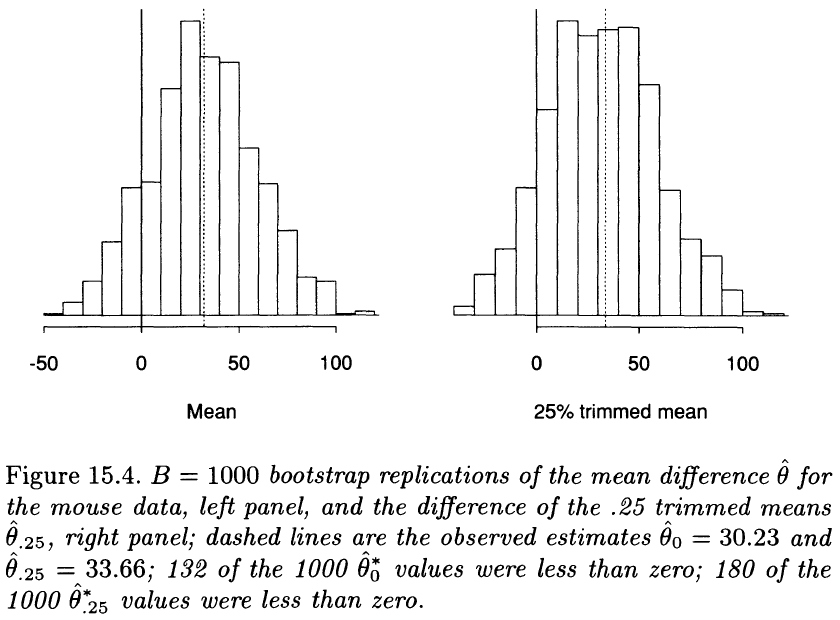
\includegraphics[width=\linewidth]{15/f15.4.png}
\newline

• Перестановочный ASL является точным, тогда как бутстреп ASL является приблизительным. Однако на практике оба метода часто дают очень похожие результаты, как в данном случае.

• Гистограммы бутстрепа центрированы около 0, в то время как гистограммы перестановок сосредоточены около 0. В этом смысле, $\text{ASL}_\text{perm}$ измеряет, насколько далека наблюдаемая оценка $\hat{\theta}$ от 0, в то время как бутстреп ASL измеряет, насколько далек 0 от $\hat{\theta}$. $\text{BC}_\text{a}$-метод, относящийся к методу процентилей (15.34) по сравнению с (15.31), предназначен для согласования этих двух способов измерения статистического «расстояния».

• Бутстреп ASL проверяет нулевую гипотезу $\theta = 0$, а перестановочный ASL проверяет $F = G$. Последний более особенный, чем первый, и иногда может показаться нереалистичным. Для данных о мышах мы могли бы проверить гипотезу о том, что средние значения двух групп равны, $\theta_0 = 0$, даже не будучи уверенными, например, в том, что два распределения имеют одинаковую дисперсию. Это скорее теоретическое возражение, нежели практическое возражение против перестановочных тестов, которые обычно работают достаточно хорошо, даже если $F = G$ является далеко не самой разумной нулевой гипотезой.

• Стандартное отклонение перестановочного распределения \textit{не} является надежной оценкой стандартной ошибки для $\hat{\theta}$ (оно не предназначено для этого), в то время как бутстреп стандартное отклонение является. В таблице 15.4 показаны стандартные отклонения перестановочного распределения и бустреп распределения данных о мышах\\
\noindent
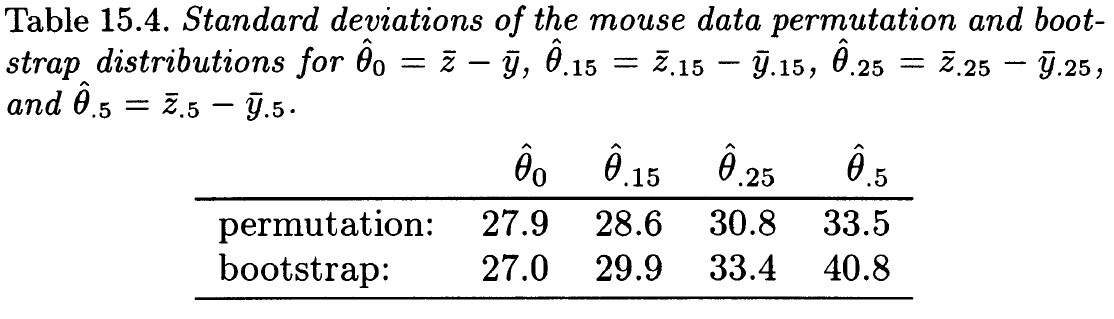
\includegraphics[width=\linewidth]{15/t15.4.png}
\newline\\
\noindent для $\hat{\theta}_0 = \bar{z} - \bar{y}, \hat{\theta}_{0.15} = \bar{z}_{0.15} - \bar{y}_{0.15}, \hat{\theta}_{0.25} = \bar{z}_{0.25} - \bar{y}_{0.25}, \hat{\theta}_{0.5} = \bar{z}_{0.5} - \bar{y}_{0.5}$. Бутстреп числа показывают более быстрое увеличение стандартной ошибки при увеличении пропорции обрезки от 0 до 0.5.

• Комбинация точечной оценки и доверительного интервала обычно более информативна, чем просто проверка гипотезы сама по себе. В эксперименте на мышах значение $\widehat{\text{ASL}}_\text{perm} = 0.132$ говорит нам только о том, что мы не можем исключить $\theta = 0$. На левой части рисунка 15.4 показано, что истинное среднее лежит между -14.5 и 73.8 с достоверностью 0.90, метод $\text{BC}_{\text{a}}$. По опыту авторов, проверка гипотез, как правило, используются чрезмерно, а доверительные интервалы --- недостаточно в статистических приложениях.

Перестановочные методы, как правило, применимы только к узкому кругу задач. Однако когда они применяются, как при тестировании $F = G$ в задаче с двумя выборками, они дают точные ответы без параметрических предположений. Первоначально бутстреп распределение называлось «комбинированным распределением». Оно было разработано, чтобы расширить возможности перестановочного тестирования для большего охвата статистических задач, где нечего переставлять. Когда есть что-то, что нужно переставить, как на рис. 15.1, это хорошая идея, даже если задействуются и другие методы, такие как бутстреп. В следующей главе мы обсудим задачи, для которых метод перестановки не может быть применен, но бутстреп проверка гипотезы все еще может быть использована.